% 轴对称基本图：对称轴 l + 对应点 A,A'，连线 AA' ⊥ l 且被 l 平分；再加一对 B,B'
\documentclass[tikz,border=4pt]{standalone}
\usepackage{ctex}
\usepackage{amsmath}
\usetikzlibrary{calc, decorations.markings}
\begin{document}
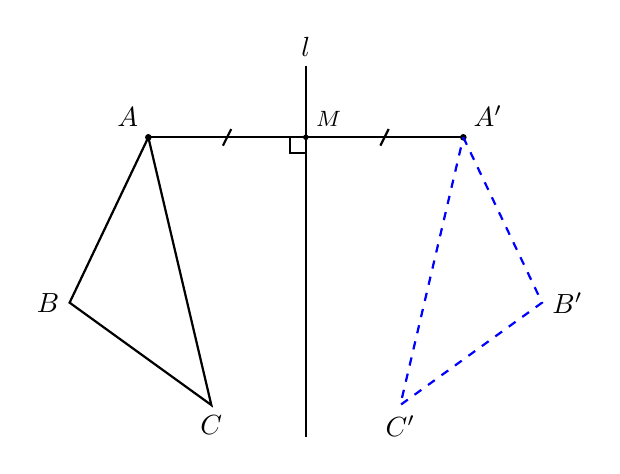
\begin{tikzpicture}[scale=1.0, thick,
  tickone/.style={postaction={decorate, decoration={markings,
    mark=at position 0.5 with {\draw (-1.5pt,-3pt) -- (1.5pt,3pt);}}}}]
  % 对称轴 l：竖直线 x=0
  \draw[thick] (0,-2.2) -- (0,2.5) node[above]{$l$};
  % 一对对应点 A(-2,1.6) ↔ A'(2,1.6)
  \coordinate (A) at (-2,1.6);
  \coordinate (Ap) at (2,1.6);
  \coordinate (MA) at (0,1.6);
  \draw[tickone] (A) -- (MA);
  \draw[tickone] (MA) -- (Ap);
  % 垂直小方块
  \draw (-0.2,1.6) -- (-0.2,1.4) -- (0,1.4);
  \fill (A) circle (1.2pt); \fill (Ap) circle (1.2pt); \fill (MA) circle (1.0pt);
  \node[above left]  at (A)  {$A$};
  \node[above right] at (Ap) {$A'$};
  \node[above right] at (MA) {\footnotesize $M$};
  % 一个三角形：A,B,C 与镜像 A',B',C'
  \coordinate (B) at (-3,-0.5);
  \coordinate (C) at (-1.2,-1.8);
  \coordinate (Bp) at (3,-0.5);
  \coordinate (Cp) at (1.2,-1.8);
  \draw (A) -- (B) -- (C) -- cycle;
  \draw[blue,dashed] (Ap) -- (Bp) -- (Cp) -- cycle;
  \node[left] at (B) {$B$};
  \node[below] at (C) {$C$};
  \node[right] at (Bp) {$B'$};
  \node[below] at (Cp) {$C'$};
\end{tikzpicture}
\end{document}
